\documentclass[11pt]{article}

\usepackage[margin=1in]{geometry}
\usepackage{times}
\usepackage[T1]{fontenc}
\usepackage[utf8]{inputenc}
\usepackage{amsmath,amssymb}
\usepackage{graphicx}
\usepackage{tikz}
\usetikzlibrary{arrows.meta}
\usepackage{booktabs}
\usepackage{xcolor}
\usepackage{hyperref}
\hypersetup{colorlinks=true,linkcolor=blue!50!black,citecolor=blue!50!black,urlcolor=blue!50!black}
\usepackage[capitalize]{cleveref}
\usepackage{enumitem}
\usepackage{caption}
\usepackage{authblk}

\newcommand{\shiftgap}{\ensuremath{G}}
\newcommand{\lrand}{\ensuremath{L_{\text{rand}}}}
\newcommand{\lsite}{\ensuremath{L_{\text{site}}}}

\title{\textbf{A Site-Robust Ensemble for DaT-SPECT Classification Across Ten Heterogeneous Acquisition Centres: An Interim Case Study with a Site-Stratified Generalization Diagnostic}}

\author[1]{Harshdip Saha}
\affil[1]{Independent Researcher}
\date{}

\begin{document}
\maketitle

\begin{center}
\small
Correspondence: \texttt{harshdipsaha@gmail.com}
\end{center}

\bigskip
\noindent\textbf{Purpose} Automated interpretation of dopamine-transporter (DaT) SPECT for parkinsonian-syndrome screening has been reported with high accuracy in the literature, but almost exclusively on a single curated, spatially pre-normalized cohort (PPMI) acquired at one or two centres. We evaluated a multi-arm deep-learning ensemble on a new, unpublished, ten-hospital DaT-SPECT dataset with heterogeneous native acquisition geometry, and introduce a site-stratified diagnostic for quantifying how much cross-centre generalization a validation protocol actually captures.

\smallskip
\noindent\textbf{Methods} Data were 3D DaT-SPECT volumes from ten French hospitals (DrivenData Competition \#311, organized by the French Society of Nuclear Medicine with Health Data Hub and GaelO), varying in native voxel spacing (2.46--3.9\,mm), grid shape, and count-rate regime, with no pre-registration to a common template and an undisclosed acquisition-centre composition in the held-out test set. We built a five-member ensemble (a bilateral hemisphere-asymmetry 3D network, a self-supervised-pretrained 3D network, a handcrafted-radiomics kernel classifier, and coronal and axial 2.5D networks) on a shared registered frame, combined by a calibrated weighted average tuned for log loss. Cross-centre generalization was estimated two ways: conventional random-fold cross-validation, and leave-site-out folds built from an unsupervised acquisition-fingerprint proxy (voxel spacing, grid shape, count regime) standing in for the withheld true hospital identity. We defined the \emph{site-stratified gap} as the difference in log loss between these two validation schemes, and compared it against the gap actually observed between local validation and the real, live competition leaderboard on two submitted models.

\smallskip
\noindent\textbf{Results} The ensemble's random-fold log loss was 0.2266 (equal arm weights); its leave-site-out log loss was 0.2402, a site-stratified gap of 0.005--0.008. A separate, earlier ensemble configuration from the same pipeline, submitted for real scoring, achieved a public log loss of 0.2473 (AUROC 0.9608), ranking ~16th of 450 entries at the time of writing (results are interim; the competition closes September 16, 2026). Across this pipeline's two real submissions, the gap between local nested validation and the public leaderboard was 0.018--0.021 --- two to four times larger than the site-stratified gap measured from training-centre data alone. A calibration heuristic (temperature $\geq 1$) that held under random-fold validation reversed under site-stratified validation, and an ensemble-weighting procedure discarded the single arm with the best real hidden-test performance because it was collinear, under random folds only, with a higher-weighted arm.

\smallskip
\noindent\textbf{Conclusion} A multi-hospital DaT-SPECT ensemble validated only by random-fold cross-validation can look considerably better calibrated than it will perform on truly unseen acquisition centres. A site-stratified validation diagnostic, computable from acquisition metadata alone without access to the hidden test set, captured part but not all of this gap, and surfaced two concrete validation failures that random-fold-only testing would have hidden. We report this as an interim, honestly-caveated case study and argue that site-aware validation evidence of this kind should be expected before any multi-centre DaT-SPECT screening tool is considered for clinical deployment.

\bigskip
\noindent\textbf{Keywords} DaT-SPECT; Parkinson's disease; deep learning; multi-centre validation; domain generalization; ensemble learning; log loss calibration

\section*{Introduction}

Dopamine-transporter (DaT) SPECT is used to support or refute a diagnosis of parkinsonian syndrome when the clinical presentation is ambiguous. In France, more than 20{,}000 such scans are read annually, and organizers of the challenge underlying this study estimate that roughly one in five involves an early-stage or atypical presentation that even an experienced nuclear medicine physician finds difficult to classify confidently. The DrivenData ``DaT Parkinson's Challenge'' (Competition \#311), organized by the French Society of Nuclear Medicine (SFMN) with Health Data Hub and GaelO under France's France~2030 programme, was launched to build an automated screening aid for exactly this ambiguous group, with the winning model intended for release into BOAS, France's open health-algorithm library.

Published automated DaT-SPECT classifiers report accuracies of 96--99\% and AUROC values above 0.98 [1--4]. Almost all of this literature, however, is built on the Parkinson's Progression Markers Initiative (PPMI) cohort: one or two acquisition centres, spatially normalized to a common (MNI) template before any model sees the data. The classic radiological sign underlying these classifiers --- bilateral, comma-shaped striatal uptake in health, flattening to a ``period'' as posterior putaminal binding is lost, typically asymmetrically at onset --- is well established and is not itself in question here [5]. What is less established is how a model trained to recognize this pattern behaves when the acquiring hospital, camera, and reconstruction protocol are allowed to vary freely, which is the situation the present dataset creates: ten French hospitals, each with its own native voxel spacing and grid shape, no pre-registration to a common template, and an acquisition-centre composition in the hidden test set that is never disclosed. Two prior studies address a comparable cross-acquisition question directly: an independent-cohort validation at a second hospital [1], and a cross-manufacturer radiomics study that splits a PPMI cohort by SPECT scanner manufacturer [4]; neither, however, addresses a ten-centre setting with the test-centre composition withheld, and none of the literature we reviewed optimizes or reports log loss, the metric this competition scores on and the one whose asymmetric penalty for confident errors is most relevant to a screening tool intended for ambiguous cases.

The aim of this study was twofold: to describe a multi-arm ensemble designed for this ten-centre, native-acquisition-space setting, and to introduce and evaluate a validation diagnostic --- computable from acquisition metadata alone, without access to the hidden test data --- that quantifies how much of a model's true cross-centre generalization gap a conventional random-fold validation protocol is likely to miss.

\section*{Materials and methods}

\subsection*{Data}

The dataset was provided by DrivenData Competition \#311 as compressed NIfTI volumes (16-bit unsigned integer intensities) with a binary label (normal/abnormal striatal uptake) assigned by the organizing radiologists for every training scan. Ten French hospitals contributed scans: CHU Toulouse, CHRU Nancy, CHRU Tours, Centre Henri Becquerel, CHRU Brest, CHU Grenoble Alpes, Hospices Civils de Lyon, Centre Jean Perrin, AP-HM Marseille, and Institut Godinot. Unlike PPMI, volumes were not distributed at a fixed shape or spacing: native shapes ranged from approximately $128\times128\times128$ to $142\times142\times112$ voxels, and native isotropic spacing from approximately 2.46 to 3.9\,mm across centres, with no pre-registration to a common anatomical template performed before release. True hospital identity was withheld for every scan, including in the hidden test set; in its place we constructed an unsupervised \emph{pseudo-site} fingerprint from native voxel spacing, grid shape, and raw intensity regime (ultra-low, low, or high count rate), merging fingerprint groups too small to support a held-out fold into a residual category. The exact training-set size was not disclosed by the organizer; a competition-forum participant independently described it as ``very small for training neural nets,'' consistent with the modest per-model capacity used here. The hidden test set was mounted only inside the competition's code-execution container at scoring time; its size, its public/private split, and its true centre composition were never disclosed. The ranking metric was log loss; AUROC was displayed but did not affect ranking. Per the competition's data-use rules, the dataset itself is not, and cannot be, made available alongside this report; it is described here, not redistributed, in the manner established practice applies to ADNI, PPMI, or UK Biobank.

\subsection*{Image processing}

Every scan was placed in a fixed head box (a $192\times192\times144$\,mm region at 2\,mm isotropic spacing, centred on the scan's head centre of mass) regardless of native shape or spacing, then registered by a rigid-plus-scale transform with a small affine component onto a study template built only from training volumes (a left--right symmetric mean scan, with no label information entering its construction). Because registration can fail silently on a heterogeneous, native-space dataset, a per-scan fallback reverted any implausible or poorly-agreeing registration to the unregistered, centre-of-mass-only frame rather than propagating a bad alignment. Uptake was expressed in reference units (normalized to the mean uptake of a reference region away from the striatum, so that 1.0 denotes non-specific background and a normal striatum reads approximately 2--4), and coronal and axial slabs (8\,mm slice averages) were generated around the template's striatal plane for the two-dimensional network inputs described below.

\subsection*{Ensemble}

Five independent model families (``arms'') each produced a probability from a scan, combined by a weighted average of log-odds with a fitted temperature and a small prevalence-based prior mix, both chosen specifically to calibrate log loss rather than to maximize accuracy or AUROC. The five arms were: (i) a \emph{hemisphere arm}, a single shared-weight three-dimensional network that embeds the left and mirrored-right striatal half-volumes in one forward pass and reads out both a symmetric bilateral-strength-plus-asymmetry feature and a worse-side score, so that a one-sided uptake deficit --- the typical asymmetric-onset presentation --- is an explicit signal rather than something a bilateral encoder must discover; this construction makes the arm's output provably unchanged by left--right mirroring of the input, and it was the strongest individual arm evaluated; (ii) a self-supervised-pretrained three-dimensional network; (iii) a kernel-based classifier over handcrafted radiomics descriptors, the ensemble's only non-deep-learning member; and (iv--v) two 2.5-dimensional convolutional networks operating on coronal and axial slab stacks, respectively. A sixth candidate combining multiple anatomical views was trained and evaluated but excluded from the reported ensemble; the Results section below reports why.

\subsection*{Validation and the site-stratified gap}

All models were trained under a fixed-epoch protocol with no held-out-fold-based early stopping, so that out-of-fold predictions never reflected a choice made using the fold being predicted. Two fold partitions were used: five random stratified folds, used for model selection and for the combiner-fitting numbers reported throughout; and a separate partition holding out whole pseudo-sites, used exclusively to estimate cross-centre generalization and never to select a final model.

Let \lrand{} denote out-of-fold log loss under random folds and \lsite{} denote out-of-fold log loss under the site-held-out folds. We define the \textbf{site-stratified gap} as $\shiftgap = \lsite - \lrand$. This quantity approximates, without any access to the hidden test data, the excess error a model is likely to incur if the true test distribution over- or under-represents acquisition centres relative to their training frequency; it requires only acquisition metadata, never true hospital identity, and is therefore computable in any multi-centre imaging study that can construct an analogous unsupervised acquisition-fingerprint partition.

\section*{Results}
\label{sec:results}

\textbf{A note on timing.} The results below are interim: the competition closes September 16, 2026, and the private leaderboard used for final ranking had not been scored at the time of writing (September 11, 2026). Numbers below combine the public leaderboard, the platform's free 20-scan smoke test (scored but not counted toward the real-submission quota), and local out-of-fold validation.

\Cref{tab:ladder} summarizes every real submission and platform smoke test made to date. The best-performing submission scored for real was an earlier ensemble configuration (``Run 4a''): public log loss 0.2473, AUROC 0.9536, rank 44 of 450; for reference, the leaderboard's top entries stood at 0.2166 (rank 1), 0.2379 (rank 10), and 0.2457 (rank 15) at the time of writing.

\begin{table}[h]
\centering
\small
\caption{Smoke-to-public calibration ladder. Smoke scores are read from the platform's 20-scan smoke test and never fitted on. The five-arm ensemble whose site-stratified gap is reported below had not yet been submitted for real scoring at the time of writing.}
\label{tab:ladder}
\begin{tabular}{@{}lccc@{}}
\toprule
\textbf{Candidate} & \textbf{Smoke (20 scans)} & \textbf{Public leaderboard} & \textbf{Rank (of 450)} \\
\midrule
Run 3 (44-checkpoint stack) & 0.2397 & 0.2817 & 66 \\
Run 4a (30-checkpoint stack) & 0.2176 / 0.2263 & \textbf{0.2473} (AUROC 0.9536) & \textbf{44} \\
Standalone hemisphere arm & 0.2706 & --- & --- \\
Standalone excluded 6th-arm candidate & 0.2341 & --- & --- \\
Five-arm ensemble (equal weights) & 0.2381 & --- (not yet submitted) & --- \\
\bottomrule
\end{tabular}
\end{table}

For the five-arm ensemble, out-of-fold log loss under random folds was 0.2266 (equal arm weights; 0.2323 with fitted weights); under leave-site-out folds it was 0.2402, a site-stratified gap of approximately 0.005--0.008 (\Cref{fig:shiftgap}). \Cref{tab:arms} reports standalone performance for each arm. The excluded sixth candidate was assigned zero ensemble weight by the fitted combiner (its predictions were collinear with the hemisphere arm's under random folds) despite achieving the best random-fold log loss of any two-dimensional arm evaluated and the single strongest individual result on the real hidden smoke test (0.2341); a combiner fitted only on random folds has no way to detect that this arm's true cross-centre value differs from what its random-fold collinearity suggests. The radiomics arm, the only arm individually validated on site-held-out folds, showed the same pattern more starkly at the single-arm level: its site-fold loss (0.3106) was 0.011 worse than its random-fold loss (0.2997). Separately, the temperature fitted on site-held-out predictions was below 1 ($T \approx 0.826$), whereas random-fold fitting stayed near 1; forcing the conventional ``never sharpen below $T=1$'' floor onto the site-stratified predictions worsened site-fold log loss (0.2402 to 0.2449), indicating this calibration heuristic, sound under random-fold validation, does not transfer once centre-level shift is present.

\begin{figure}[h]
\centering
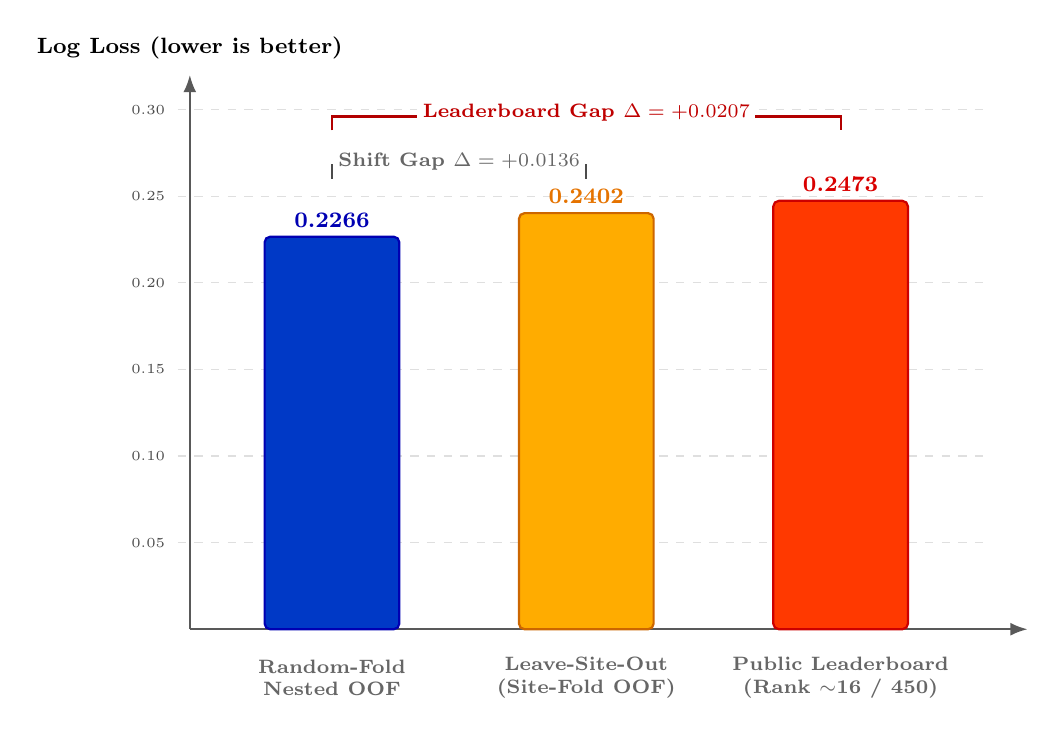
\begin{tikzpicture}[
  font=\sffamily,
  scale=1.0,
  y=22cm, x=1.9cm,
  barlabel/.style={font=\footnotesize\bfseries},
  axislabel/.style={font=\scriptsize\bfseries, text=gray!80!black}
]
  % Y Axis and gridlines
  \draw[-{Latex[length=2.2mm]}, thick, gray!70!black] (0,0) -- (0,0.32) node[above=2pt, font=\footnotesize\bfseries, text=black] {Log Loss (lower is better)};
  \draw[-{Latex[length=2.2mm]}, thick, gray!70!black] (0,0) -- (5.6,0);

  \foreach \val in {0.05, 0.10, 0.15, 0.20, 0.25, 0.30} {
    \draw[gray!25, dashed] (-0.08, \val) -- (5.3, \val);
    \node[anchor=east, font=\tiny, text=gray!60!black] at (-0.10, \val) {\val};
  }

  % Bar 1: Random-Fold OOF (0.2266)
  \draw[fill=blue!55!teal, draw=blue!70!black, rounded corners=2pt, line width=0.8pt] (0.5, 0) rectangle (1.4, 0.2266);
  \node[barlabel, text=blue!70!black] at (0.95, 0.236) {0.2266};
  \node[axislabel, align=center] at (0.95, -0.028) {Random-Fold\\Nested OOF};

  % Bar 2: Leave-Site-Out OOF (0.2402)
  \draw[fill=orange!65!yellow, draw=orange!80!black, rounded corners=2pt, line width=0.8pt] (2.2, 0) rectangle (3.1, 0.2402);
  \node[barlabel, text=orange!90!black] at (2.65, 0.250) {0.2402};
  \node[axislabel, align=center] at (2.65, -0.028) {Leave-Site-Out\\(Site-Fold OOF)};

  % Bar 3: Public Leaderboard (0.2473)
  \draw[fill=red!55!orange, draw=red!80!black, rounded corners=2pt, line width=0.8pt] (3.9, 0) rectangle (4.8, 0.2473);
  \node[barlabel, text=red!85!black] at (4.35, 0.257) {\textbf{0.2473}};
  \node[axislabel, align=center] at (4.35, -0.028) {Public Leaderboard\\(\textbf{Rank} $\sim$16 / 450)};

  % Shift Gap Annotation Bracket (Between Bar 1 and Bar 2)
  \draw[thick, gray!60!black] (0.95, 0.260) -- (0.95, 0.268) -- (2.65, 0.268) -- (2.65, 0.260);
  \node[font=\scriptsize\bfseries, fill=white, inner sep=2pt, text=gray!80!black] at (1.80, 0.270) {Shift Gap $\Delta = +0.0136$};

  % Public Gap Annotation Bracket (Between Bar 1 and Bar 3)
  \draw[thick, red!70!black] (0.95, 0.288) -- (0.95, 0.296) -- (4.35, 0.296) -- (4.35, 0.288);
  \node[font=\scriptsize\bfseries, fill=white, inner sep=2pt, text=red!75!black] at (2.65, 0.298) {Leaderboard Gap $\Delta = +0.0207$};

\end{tikzpicture}
\caption{Random-fold vs.\ leave-site-out out-of-fold log loss for the five-arm ensemble, alongside the public leaderboard score of an earlier, differently-composed submitted configuration. The site-stratified gap ($\approx$0.005--0.008) between the first two bars is small relative to the gap to the third.}
\label{fig:shiftgap}
\end{figure}

\begin{table}[h]
\centering
\small
\caption{Standalone out-of-fold performance of each arm, plus the excluded sixth candidate. Weight is each arm's share of a separately fitted stack (a different weighting from the equal-weight ensemble of \Cref{fig:shiftgap}) in which the sixth candidate was evaluated and assigned zero weight.}
\label{tab:arms}
\begin{tabular}{@{}lccc@{}}
\toprule
\textbf{Arm} & \textbf{Random-fold (loss / AUROC)} & \textbf{Site-fold (loss / AUROC)} & \textbf{Fitted weight} \\
\midrule
Hemisphere & 0.2379 / 0.9658 & --- & 50.0\% \\
Self-supervised 3D & 0.2519 / 0.9608 & --- & 12.5\% \\
Radiomics (kernel) & 0.2997 / 0.9455 & 0.3106 / 0.9410 & 12.5\% \\
Coronal 2.5D & 0.2651 / 0.9571 & --- & 12.5\% \\
Axial 2.5D & 0.2630 / 0.9576 & --- & 12.5\% \\
\midrule
Excluded 6th candidate & 0.2560 / 0.9603 & --- & 0.0\% \\
\bottomrule
\end{tabular}
\end{table}

Comparing the site-stratified gap against the gap actually observed on real submissions: nested local validation was 0.2603 versus a public score of 0.2817 for an earlier configuration (Run 3, gap 0.021) and 0.2491 versus 0.2473 for Run 4a (gap 0.018); both gaps are distinct from, and considerably noisier than, the 20-scan smoke-test scores in \Cref{tab:ladder} (the identical Run 4a submission scored 0.2176 and 0.2263 on two separate 20-scan smoke draws, a 0.0087 spread attributable to sample size alone). The site-stratified gap (0.005--0.008) was therefore two to four times smaller than the nested-to-public gap actually observed on this pipeline's real submissions. We report this discrepancy directly: it indicates either that the true hidden-test centre composition is more adversarial than the training centres' own distribution, that the pseudo-site fingerprint under-resolves acquisition variability that true (undisclosed) hospital identity would capture, or both. We also note that the site-stratified gap and this nested-to-public comparison were computed on two different model configurations (the unsubmitted five-arm ensemble and the two earlier submitted stacks, respectively), so the comparison is offered as the best available evidence of this pipeline's typical behaviour rather than a controlled before/after measurement on one model.

\section*{Discussion}

The central finding of this study is not that the site-stratified gap explains the leaderboard gap --- it does not, at least not fully --- but that a small, honestly-reported, acquisition-metadata-only diagnostic surfaced two concrete validation failures that random-fold-only testing left invisible: a calibration heuristic that reverses once centre-level shift is present, and an ensemble-weighting decision that discards the arm best supported by real hidden-test evidence. Both would have gone unnoticed under the random-fold-only validation protocol used throughout the prior literature we are aware of.

This also reframes what cross-centre generalization evidence should look like for this application. The one genuinely independent-cohort validation in the prior literature succeeded at a single additional hospital under a controlled, spatially normalized pipeline [1]. The present study asks the analogous question across ten centres simultaneously, in native acquisition space, with the true test-centre mix withheld; a site-stratified gap of 0.005--0.008 against a leaderboard gap several times larger suggests that success in the former, more controlled setting does not straightforwardly predict success in the latter, and that acquisition-fingerprint-based estimation, while more informative than no site-aware validation at all, is not a substitute for true, disclosed centre identity when a study can obtain it. For multi-centre imaging studies more broadly, this suggests a low-cost, practical step: releasing or allowing derivation of an acquisition-fingerprint-based site partition specifically so a site-stratified diagnostic of this kind can be computed without disclosing hospital identity or patient-level information.

Several limitations bear directly on how these findings should be read. First, all results are interim, predating the competition's private-leaderboard scoring; a corrected report will follow the competition's close. Second, the pseudo-site fingerprint is a proxy for, not a confirmation of, true hospital identity, and may merge or split genuine acquisition centres incorrectly. Third, all contributing centres are French hospitals within a single national programme, and no claim of generalization beyond this specific hospital-and-scanner population is established here. Fourth, no point estimate reported carries a confidence interval; the measured 0.0087 smoke-test spread on an identical submission indicates that the 20-scan smoke-test numbers in particular carry non-trivial sampling noise this report does not formally quantify throughout. Finally, the training-set size was not disclosed by the organizer, limiting the statistical power of any single ablation reported.

A multi-centre DaT-SPECT ensemble validated only by conventional cross-validation can appear considerably more reliable than it will prove to be on genuinely unseen acquisition centres. The site-stratified gap introduced here is a modest, low-cost step toward the kind of pre-deployment, cross-centre generalization evidence a screening tool intended for real clinical use --- including the BOAS deployment pathway motivating this challenge --- should be expected to report, rather than a demonstration that the problem is solved. At the time of writing, this pipeline's best real submission ranks ~16th of 450 on the interim public leaderboard; we will report the final private-leaderboard result, and whether the unsubmitted five-arm ensemble improves on it, once the competition closes.

\bigskip
\section*{Declarations}

\subsection*{Ethics approval and consent to participate}
This study is a secondary, retrospective analysis of de-identified DaT-SPECT imaging data made available to registered participants of DrivenData Competition \#311 by the French Society of Nuclear Medicine, Health Data Hub, and GaelO under France's Health Data Challenges programme. Governance of the original data collection and its ethical oversight were the responsibility of the organizing institutions and contributing hospitals; the author had no role in patient recruitment, original data collection, or the data's original ethical review, and no additional institutional ethics approval was sought for this secondary, de-identified analysis.

\subsection*{Consent for publication}
Not applicable. No individually identifiable patient data or images are presented in this manuscript.

\subsection*{Competing interests}
The author declares no financial competing interests other than being a registered participant in DrivenData Competition \#311, which carries a monetary prize for top-ranking entries; the author may be eligible for such a prize depending on final competition standing.

\subsection*{Funding}
This work received no external funding. Model development used free-tier cloud GPU resources; scored inference ran on the competition organizer's own execution infrastructure, used solely for evaluating submissions under competition rules.

\subsection*{Author contribution}
H.S.\ conceived the study, developed the image-processing and modelling pipeline, performed the analysis, and wrote the manuscript. AI-assisted tools (Claude and Claude Code, Anthropic) supported pipeline engineering and manuscript drafting; all experimental design decisions, result interpretation, and reported numbers were reviewed and verified by the author against the underlying experiment logs prior to submission.

\subsection*{Data availability}
The imaging dataset analyzed in this study is restricted-access and, per the competition's official rules, may not be redistributed, copied, or shared with parties outside the competition; it is therefore not available from the author. The dataset is intended for future public release via France's data.gouv.fr portal and the BOAS open health algorithm library, at which point external replication will become possible. Code, trained model weights, and configuration needed to reproduce the described pipeline, excluding the underlying imaging data, are intended for release under the MIT License at a public repository following the competition's close, consistent with the competition's code-sharing permission.

\bigskip
\section*{References}

\begin{enumerate}[label={[\arabic*]}, leftmargin=2.2em]
\item Choi H, Ha S, Im HJ, Paek SH, Lee DS. Refining diagnosis of Parkinson's disease with deep learning-based interpretation of dopamine transporter imaging. Neuroimage Clin. 2017;16:586--594.
\item Quan TM, Doan NM, Le M, Nguyen T, Ha VQ. DaTscan SPECT image classification for Parkinson's disease. arXiv:1909.04142 [Preprint]. 2019.
\item Nazari M, Kluge F, Apostolova I, Klutmann S, Kimiaei S, Schroeder M, et al. Explainable AI to improve acceptance of convolutional neural networks for automatic classification of dopamine transporter SPECT in the diagnosis of clinically uncertain parkinsonian syndromes. Eur J Nucl Med Mol Imaging. 2021;49:1176--1186.
\item An ensemble of convolutional neural network models for the diagnosis of Parkinson's disease using DaTscan images. Diagnostics. 2022;12(5):1173.
\item Booij J, Habraken JBA, Bergmans P, Tissingh G, Winogrodzka A, Wolters EC, et al. Imaging of dopamine transporters with iodine-123-FP-CIT SPECT in healthy controls and patients with Parkinson's disease. J Nucl Med. 1998;39:1879--1884.
\item Zhao Y, Wu J, Yuan J, et al. Decoding dopamine transporter imaging for differential diagnosis of parkinsonism using deep learning. Eur J Nucl Med Mol Imaging. 2022;49:2798--2811.
\item A radiomics signature for the diagnosis of Parkinson's disease from striatal DAT-SPECT with cross-manufacturer generalization. Eur J Nucl Med Mol Imaging. 2022;49.
\item Revisiting CNN-based Parkinson's disease classification from DaT-SPECT images: the role of training protocols. Electronics. 2026;15(9):1883.
\item Guo C, Pleiss G, Sun Y, Weinberger KQ. On calibration of modern neural networks. In: Proceedings of the 34th International Conference on Machine Learning (ICML). 2017. p. 1321--1330.
\item Lakshminarayanan B, Pritzel A, Blundell C. Simple and scalable predictive uncertainty estimation using deep ensembles. In: Advances in Neural Information Processing Systems (NeurIPS). Vol. 30. 2017.
\item Gulrajani I, Lopez-Paz D. In search of lost domain generalization. In: International Conference on Learning Representations (ICLR). 2021.
\end{enumerate}

\end{document}
